\documentclass{article}
\usepackage{tikz}
\usepackage{pgfplots}
\begin{document}
	
	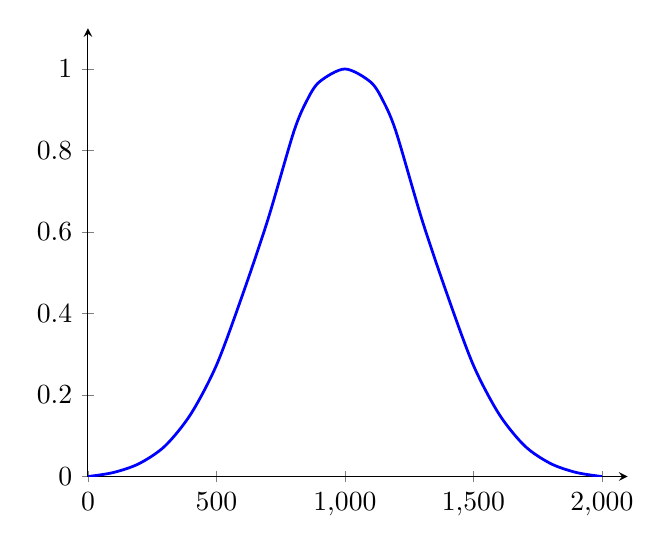
\begin{tikzpicture}
	\begin{axis}[
	axis x line=bottom,
	axis y line=left,
	ymax=1.1,xmin=0,xmax=2100]
	
	\addplot[smooth,blue,line width=1pt]
	plot coordinates {
		(0,0)
		(100,0.01)
		(200,0.032)
		(300,0.075)
		(400,0.153)
		(500,0.273)
		(600,0.443)
		(700,0.63)
		(800,0.844)
		(850,0.92)
		(900,0.968)
		(1000,1)
		(1100,0.968)
		(1150,0.92)
		(1200,0.844)
		(1300,0.63)
		(1400,0.443)
		(1500,0.273)
		(1600,0.153)
		(1700,0.075)
		(1800,0.032)
		(1900,0.01)
		(2000,0)
		
	};
	\node at (13,107) {$w(t)$};
	\node at (206,6) {$t$};
	\end{axis}
	\end{tikzpicture}
	
\end{document} 